\documentclass[10pt, a4paper]{article}

\usepackage[T1]{fontenc}
\usepackage{fullpage}
\usepackage[utf8]{inputenc}
\usepackage{siunitx}
\usepackage{tikz}
\usepackage[european]{circuitikz}
\usepackage{titlesec}

\setlength{\parindent}{0pt}

\titleformat{\section}{\normalsize\bfseries}{\thesection}{1em}{}
\titleformat{\subsection}{\normalsize\bfseries}{\thesubsection}{1em}{}
\titleformat{\subsubsection}{\normalsize\bfseries}{\thesubsubsection}{1em}{}

\begin{document}
    \begin{center}
        \large \textsc{Lattice Watering}

        \vspace{\baselineskip}

        \normalsize Handout

        \vspace{\baselineskip}

        Christian Müller, Jonas Heinemann, Kaan Dönmez, Valentin Pickel

        \vspace{\baselineskip}

        Software Project on Internet Communications
        
        Summer Term 2022

        Freie Universität Berlin

        \vspace{\baselineskip}

        July 18, 2022
    \end{center}

    \rule{\linewidth}{0.5pt}

    \section{Introduction}

    We may start from scratch by reminiscing the the first meeting of all course participants on April 4th. This software project course should dive into the ecosystem internet. To do so, a rough split was set between the worlds of the \emph{Internet of Things} (IoT), which deals with low power devices in large networks, and the conventional internet and its vastly more potent desktop computers and servers. Especially, us students should become aware of design decisions with respect to the communication solutions that our software should utilize. The project \emph{Lattice Watering} eyes out the first of both worlds.

    \subsection{Idea Outline}

    After suggesting the building an IoT application for watering plants automatically on May 2nd, the software project \emph{Lattice Watering} and its group formed on the 9th of May, comprising of the aforementioned members. The term \emph{Lattice} is a reference to the studies of crystal/grid-like molecular structures in physics settings, which are often represented by two-dimensional structures called lattices. The first idea was not just to automate the watering of the plants, but also to let the boards drive around on a large grid. As it turns out, the hardware requirements for such a project would be too difficult to implement, so after some discussion we stuck to the original idea of a plant watering application, not changing the initial name.

    In a nutshell, the idea is to be able to use a normal desktop computer to control several smaller microcontrollers, that are scattered widely. This may happen by setting automatic rules, or by the microcontrollers automatically turning on the water pumps as soon as humidity levels, which are measured by sensory, drop beyond a certain threshold. The latter aspect can be configured in a web frontend that is designed by us. Besides watering the plants, we also collect statistics like the humidity levels or network usage.

    \subsection{Team Organization and Applied Practices}

    For a detailled overview of the code hierarchy, one can look into the file \texttt{README.md} inside of the project directory.
    
    \emph{git} was used as our version control system, with a repository setup on \emph{GitHub}. Our team members usually did not have fixed tasks, but utilize the agile method of \emph{Kanban}. On GitHub, a kanban board was setup, in which members can add new issues and tasks to three categories: \emph{Backlog}, \emph{In Progress} and \emph{Done}. This allowed our work to proceed in a assembly line-type way, in the sense that there are certain tasks that are saved up for later. However, in the nature of things, some members prefer to work closer to the IoT devices themselves, whilst others work e.g. with the web frontend. It is important to mention that we used \emph{agile} methods, as we all had different experiences in the field of IoT communication we were studying, so agile methods and rapid prototyping seemed like good methods for this project.

    Our methods of work also include \emph{code conventions}, which are described in the \texttt{README.md} file. Such include using formatting tools and static analyzers, as well as code practices. Although they are quite few in this project, they reflect that we should take care of code quality at all times, and using matured automatic tools for that eases a normally adiministrative task.

    Communication was done via the proprietary communication platform \emph{Discord}, which was preferred over a decentralized solution like \emph{Element/Matrix} due to all course members already using it.

    \begin{figure}[!hbtp]
        \centering
        \includegraphics[width=\linewidth]{img/kanban_board.png}
        \caption{The kanban project board. (State: 13th June, 18:32)}
    \end{figure}

    \section{Hardware}

    \begin{figure}[htbp!]
        \centering
        \begin{circuitikz}
            \draw (0, 0) node[left] {\(\qty{92}{\milli\ampere}, \qty{3.8}{\volt}\)}
                to[R=$\qty{200}{\ohm}$, -*] (2, 0);
            \draw (2, 0)
            to[R=\(\qty{5}{\kilo\ohm}\)] (2, -2) node[ground] {};
            \draw (4, 0) node[nigfete, tr circle] (mos) {}
            (mos.source) node[anchor=north] {}
            (mos.gate) node[anchor=east] {}
            (mos.drain) node[anchor=south] {};
            \draw (mos.inner up) -- (mos.body E out);
            \draw (mos.body E out) -- (mos.body C out);
            \draw (mos.body C out) -- (mos.body C in);
            \draw (2, 0) -- (mos.gate);
            \draw (mos.source) -- (4, -2) node[ground] {};
            \draw (mos.drain) -- (4, 2) node[circle] {P};
            \end{circuitikz}
        \caption{Circuit for the pump P.}
    \end{figure}

    Thus, we obtain:
    \[
        I_2 = \frac{\qty{5}{\volt}}{\qty{200}{\ohm}} = \qty{25}{\milli\ampere}
    \]
    And:
    \[
        I_3 = \frac{\qty{5}{\volt}}{\qty{200}{\ohm}} = \qty{25}{\milli\ampere}
    \]

    \section{Network Structure}

    \begin{figure}[!hbtp]
        \centering
        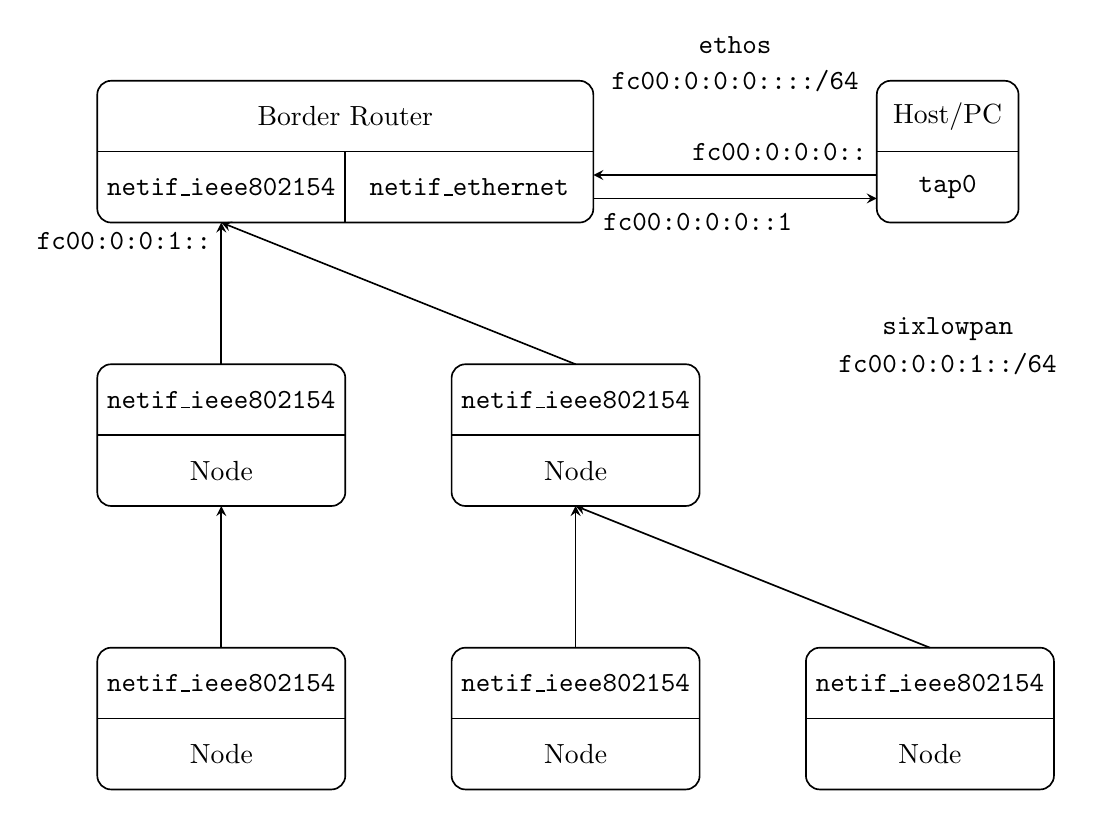
\begin{tikzpicture}[>=stealth, semithick, scale=0.9]
            \draw[rounded corners=5pt] (-1, -1) rectangle (1, 1);
            \draw[draw=none] (-1, 0) -- (1, 1) node[pos=0.5] {Host/PC};
            \draw (-1, 0) -- (1, 0);
            \draw[draw=none] (-1, 0) -- (1, -1) node[pos=0.5] {\texttt{tap0}};

            \draw[rounded corners=5pt] (-12, -1) rectangle (-5, 1);
            \draw[draw=none] (-12, 0) -- (-5, 1) node[pos=0.5] {Border Router};
            \draw (-12, 0) -- (-5, 0);
            \draw (-8.5, 0) -- (-8.5, -1);
            \draw[draw=none] (-12, 0) -- (-8.5, -1) node[pos=0.5] {\texttt{netif\_ieee802154}};
            \draw[draw=none] (-8.5, 0) -- (-5, -1) node[pos=0.5] {\texttt{netif\_ethernet}};
            \draw[->] (-1, -0.33) -- (-5, -0.33);
            \node[left] at (-1, 0) {\texttt{fc00:0:0:0::}};
            \node[right] at (-5, -1) {\texttt{fc00:0:0:0::1}};
            \node at (-3, 1.5) {\texttt{ethos}};
            \node at (-3, 1) {\texttt{fc00:0:0:0::::/64}};
            \draw[->] (-5, -0.66) -- (-1, -0.66);
            \node[below left] at (-12+1.75, -1) {\texttt{fc00:0:0:1::}};

            \newcommand{\networknode}[2]{
                \draw[rounded corners=5pt] (#1, #2) rectangle (#1+3.5, #2-2);
                \draw (#1, #2-1) -- (#1+3.5, #2-1);
                \draw[draw=none] (#1, #2) -- (#1+3.5, #2-1) node[pos=0.5] {\texttt{netif\_ieee802154}};
                \draw[draw=none] (#1, #2-1) -- (#1+3.5, #2-2) node[pos=0.5] {Node};
            }

            \networknode{-12}{-3};
            \networknode{-7}{-3};
            \networknode{-12}{-7};
            \networknode{-7}{-7};
            \networknode{-2}{-7};

            \draw[->] (-12+1.75, -3) -- (-12+1.75, -1);
            \draw[->] (-7+1.75, -3) -- (-12+1.75, -1);
            \draw[->] (-12+1.75, -7) -- (-12+1.75, -5);
            \draw[->] (-7+1.75, -7) -- (-7+1.75, -5);
            \draw[->] (-2+1.75, -7) -- (-7+1.75, -5);

            \node at (0, -2.5) {\texttt{sixlowpan}};
            \node at (0, -3) {\texttt{fc00:0:0:1::/64}};
        \end{tikzpicture}
        \caption{The Network Topology. The device interfaces are named after our code. The \texttt{tap0} device is named after the typical Linux entry. The network stack is based on COAP, DTLS, UDP, 6LoWPAN IPHC and FRAG, RPL, IPv6. The global IP addresses of the nodes inside the \texttt{fc00:0:0:0:0:0:0:1::/64} network are chosen by appending the Layer 2 addresses to the network prefix. The DAG structure of the RPL network is shown schematically.}
    \end{figure}

    \section{Application Structure}

    \section{Closing Words}

    \listoffigures
\end{document}
